\documentclass[12pt]{article}
\usepackage{enumitem}
\usepackage{graphicx}
\usepackage{amsmath}
\usepackage{fvextra}
\usepackage{hyperref}
\usepackage{subcaption}
\usepackage[title]{appendix}

\usepackage[backend=bibtex,style=ieee]{biblatex}
\addbibresource{atmos.bib}

\newcommand{\numpy}{{\tt numpy}}    % tt font for numpy

\DefineVerbatimEnvironment{Verbatim}{Verbatim}{breaklines=true}

\topmargin -.5in
\textheight 9in
\oddsidemargin -.25in
\evensidemargin -.25in
\textwidth 7in
\renewcommand{\baselinestretch}{1.3}

\begin{document}

\author{Timon Sommer}
\title{CS7GV3 Final Assignment: \\ Atmospheric Scattering}
\date{}
\maketitle

\textbf{Student ID: 24334440}

% TODO: add yt link
\textbf{Video: \url{}}

\medskip

\begin{abstract}
In this report, a method for rendering atmospheric scattering in real-time is investigated and parts of it are implemented using OpenGL and C++.
Instead of using a pre-computed look-up table (LUT) for properties of the atmosphere, the method relies on a ray-marching approach that determines the scattering of light in the atmosphere in real-time using simplifying assumptions about atmospheric transmittance.
We eventually find that the implementation is capable of producing visually plausible results at interactive frame rates, while higher iteration counts only slightly improve fidelity yet significantly decrease performance.
Additionally, the chosen approach currently ignores transparency of the atmosphere towards objects in space and remains limited to views directed from space towards the atmosphere, but can be extended to support views from the ground towards the sky.

\end{abstract}

\section{Background}
\subsection{Natural Atmospheric Scattering}
Atmospheric scattering is a phenomenon that occurs when light from space such as sun- or moonlight interacts with particles in the atmosphere, creating visual effects such as the sky appearing blue during the day and red when approaching dawn or dusk.
Depending on the kind of particle involved, there are two main scattering components as described in \cite{bruneton_precomputed_2008}:
\begin{itemize}
    \item Rayleigh scattering: This type of scattering interacts with smaller particles such as air molecules.
    Since its scattering behaviour depends on the wavelength of the light, it is responsible for the varying colour of the sky at different times of the day (see Figure \ref{fig:atmospheric_scattering}).
    \item Mie scattering: Here, light rays are scattered by bigger particles in the atmosphere such as aerosols.
    Scattering of this kind affects all wavelengths equally, which causes the sky to appear white or hazy when the sun approaches the horizon.
\end{itemize}
\begin{figure}[h!]
    \centering
    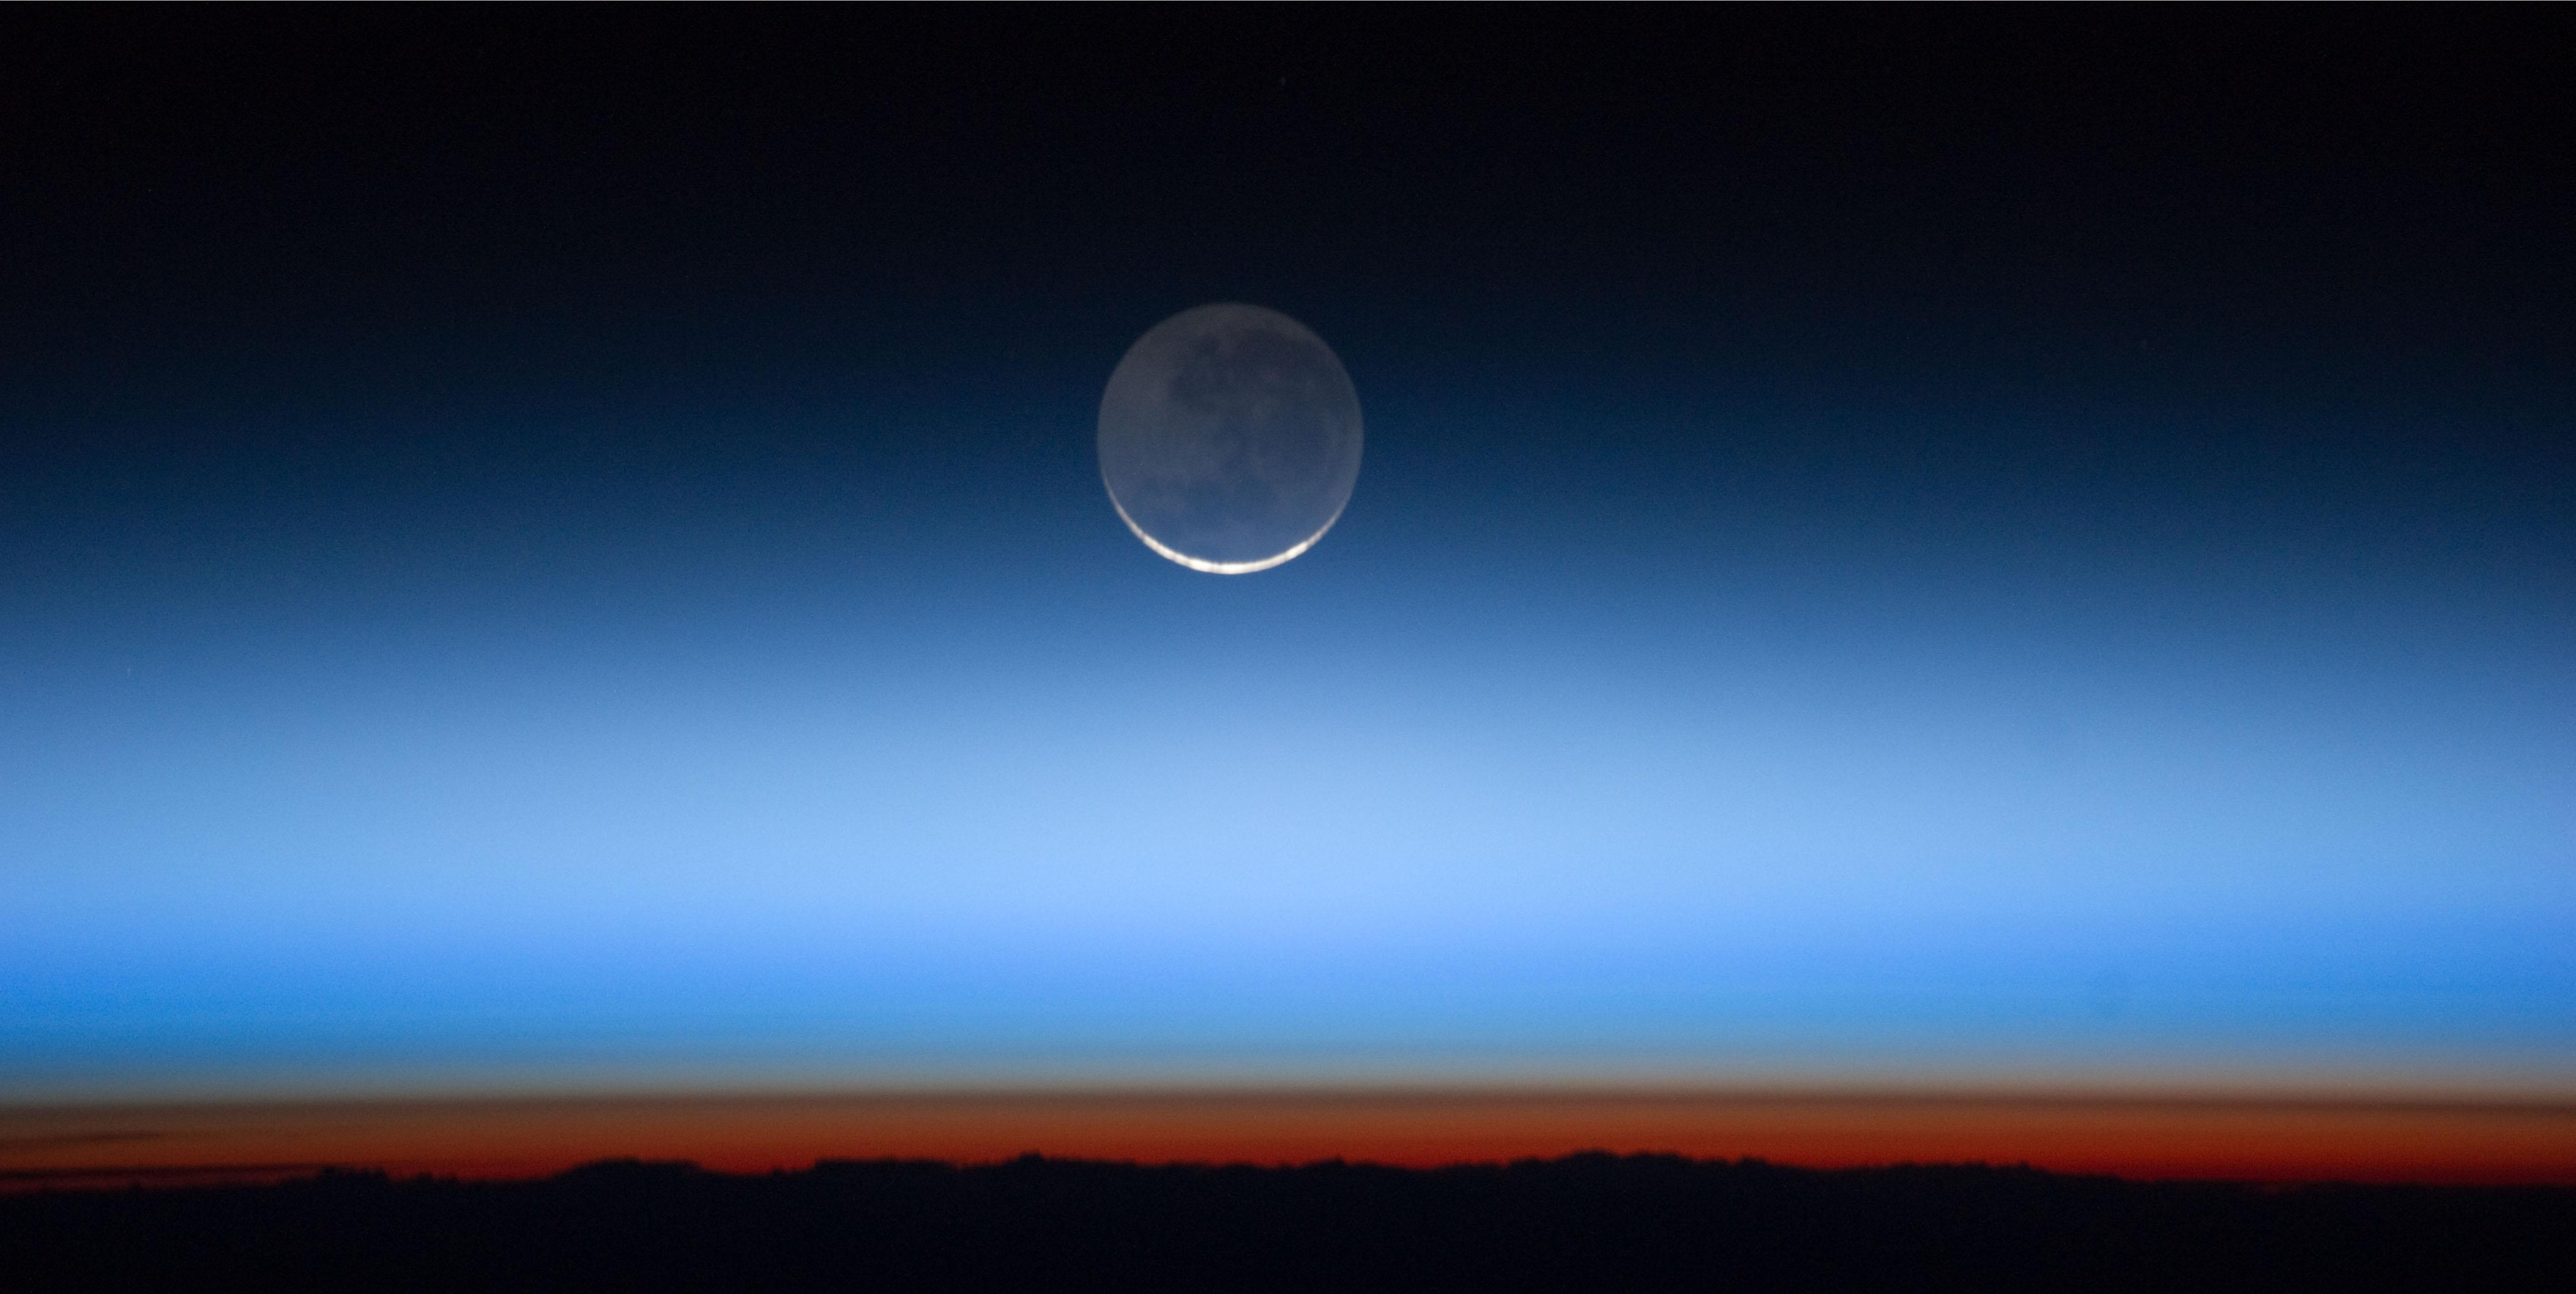
\includegraphics[width=1.0\textwidth]{./figures/atmos.jpg}
    \caption{Photograph of the atmosphere of the earth taken from space.
    \\Source: \url{https://earthobservatory.nasa.gov/images/76534/hovering-on-the-horizon}}
    \label{fig:atmospheric_scattering}
\end{figure}
\subsection{Precomputed Atmospheric Scattering}
As light rays travel through the atmosphere from the source to the viewer, light is scattered into and out of the rays along the ray trajectory, modulating the final intensity of all wavelengths.
Both the light resulting from in- and out-scattering can be described using integrals over the ray trajectory:
Due to the complexity of these processes, the approach presented \cite{bruneton_precomputed_2008} uses a pre-computed LUT to store the scattering properties of the atmosphere.
Most importantly, this LUT contains the transmittance of the atmosphere at a given height, where the values are calculated using a numerical integration of the scattering equations.
This way, the integral approximation does not need to be sampled in real-time, which would otherwise be computationally expensive.
\begin{figure}[h!]
    \centering
    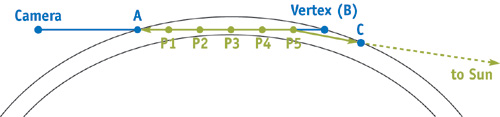
\includegraphics[width=0.5\textwidth]{./figures/ray_oneill.jpg}
    \caption{Discrete ray sampling as described in \cite{oneil_chapter_nodate}.Source: \cite{oneil_chapter_nodate}}
    \label{fig:oneill_scattering}
\end{figure}

The article \cite{oneil_chapter_nodate} implemented in this project does approximate the scattering integrals but still makes simplifying assumptions to allow evaluating both the out- and in-scattering terms at interactive frame rates.
Based on the formulation of the scattering equations in \cite{nishita_display_1993}, the author of \cite{oneil_chapter_nodate} derives the equation for the out-scattering component as
\begin{align}
    t(P_x Py, \lambda) = 4\pi \times K(\lambda) \times \int_{P_x}^{P_y} \exp\left( \frac{-h}{H_0} \right) \, ds,
    \label{eq:out}
\end{align}
where $K(\lambda)$ is the scattering coefficient dependent on the wavelength $\lambda$, $H_0$ is the altitude of the highest density in the atmosphere, and $h$ is the height of the discrete sample point above the planet surface.
We can then nest this equation inside another integral over all sample points along the ray to yield the in-scattering term as
\begin{align}
    I_v(\lambda) = I_s(\lambda) \times K(\lambda) \times F(\theta, g) \times \int_{P_a}^{P_b} \left( \exp\left( \frac{-h}{H_0} \right) \times \exp\left( -t(P_xP_c, \lambda) - t(P_xP_a, \lambda) \right) \right) \, ds,
    \label{eq:in}
\end{align}
where $I_s(\lambda)$ is the intensity of the light source, and $F(\theta, g)$ is the phase function dependent on the angle between the incident light and camera rays at each sample point (see points $P_1 - P_5$ in Figure \ref{fig:oneill_scattering}):
\begin{align}
    F(\theta, g) = \frac{3 (1 - g^2)}{2 (2 + g^2)} \cdot \frac{1 + \cos^2\theta}{\left(1 + g^2 - 2g\cos\theta\right)^{3/2}}.
    \label{eq:phase}
\end{align}
Since both $K$ and the scattering symmetry factor $g$ and thus also $F$ are different for Rayleigh and Mie scattering, contributions of both components need to be calculated separately and then added to yield the final result.

The main simplification made in \cite{oneil_chapter_nodate} is to approximate the height-related integral in equations \eqref{eq:in} and \eqref{eq:out} by fitting it to an exponential curve:
\begin{align}
    \int_{P_a}^{P_b} \exp\left( \frac{-h}{H_0} \right) \, ds \approx \exp(-4h).
    \label{eq:approx}
\end{align}
However, since this approximation is based on normalising the height $h$, it needs to be multiplied by a transformation funciton that maps the values to the actual atmosphere height range.
This polynomial transformation function is defined dependent on both $H_0$ as well as the relative distance between the surface and the outer atmosphere and thus would have to be recomputed whenever any of these parameters change.
\section{Implementation}
Given that the approach presented in \cite{oneil_chapter_nodate} requires a new transformation function to be computed whenever the atmosphere height or $H_0$ for either Rayleigh or Mie changes, the implementation in this report foregoes this step.
Inspired by the approach in \cite{gltracy_shadertoy_nodate}, the exponential optical depth term is instead approximated by evaluating the left side of equation \eqref{eq:approx} at discrete sample points along the ray trajectory.
This decision was made given that this article was published in 2005, and the capabilities of modern GPUs have improved significantly since then.

Still, the overall raymarching approach employed in \cite{oneil_chapter_nodate} is retained with the modification that it is performed in a fragment shader instead of a vertex shader.
While computationally more expensive, this leads to a higher resolution of the rendered atmosphere, especially because we assign the shader to a sphere mesh instead of a full screen quad.
This is done to keep depth testing intact without having to write manually to the depth buffer, enabling us to integrate the atmosphere shader with standard rasterisation-based shaders assigned to other objects such as the moon or the sun (see Figure \ref{fig:occlusion}).
\begin{figure}[h!]
    \centering
    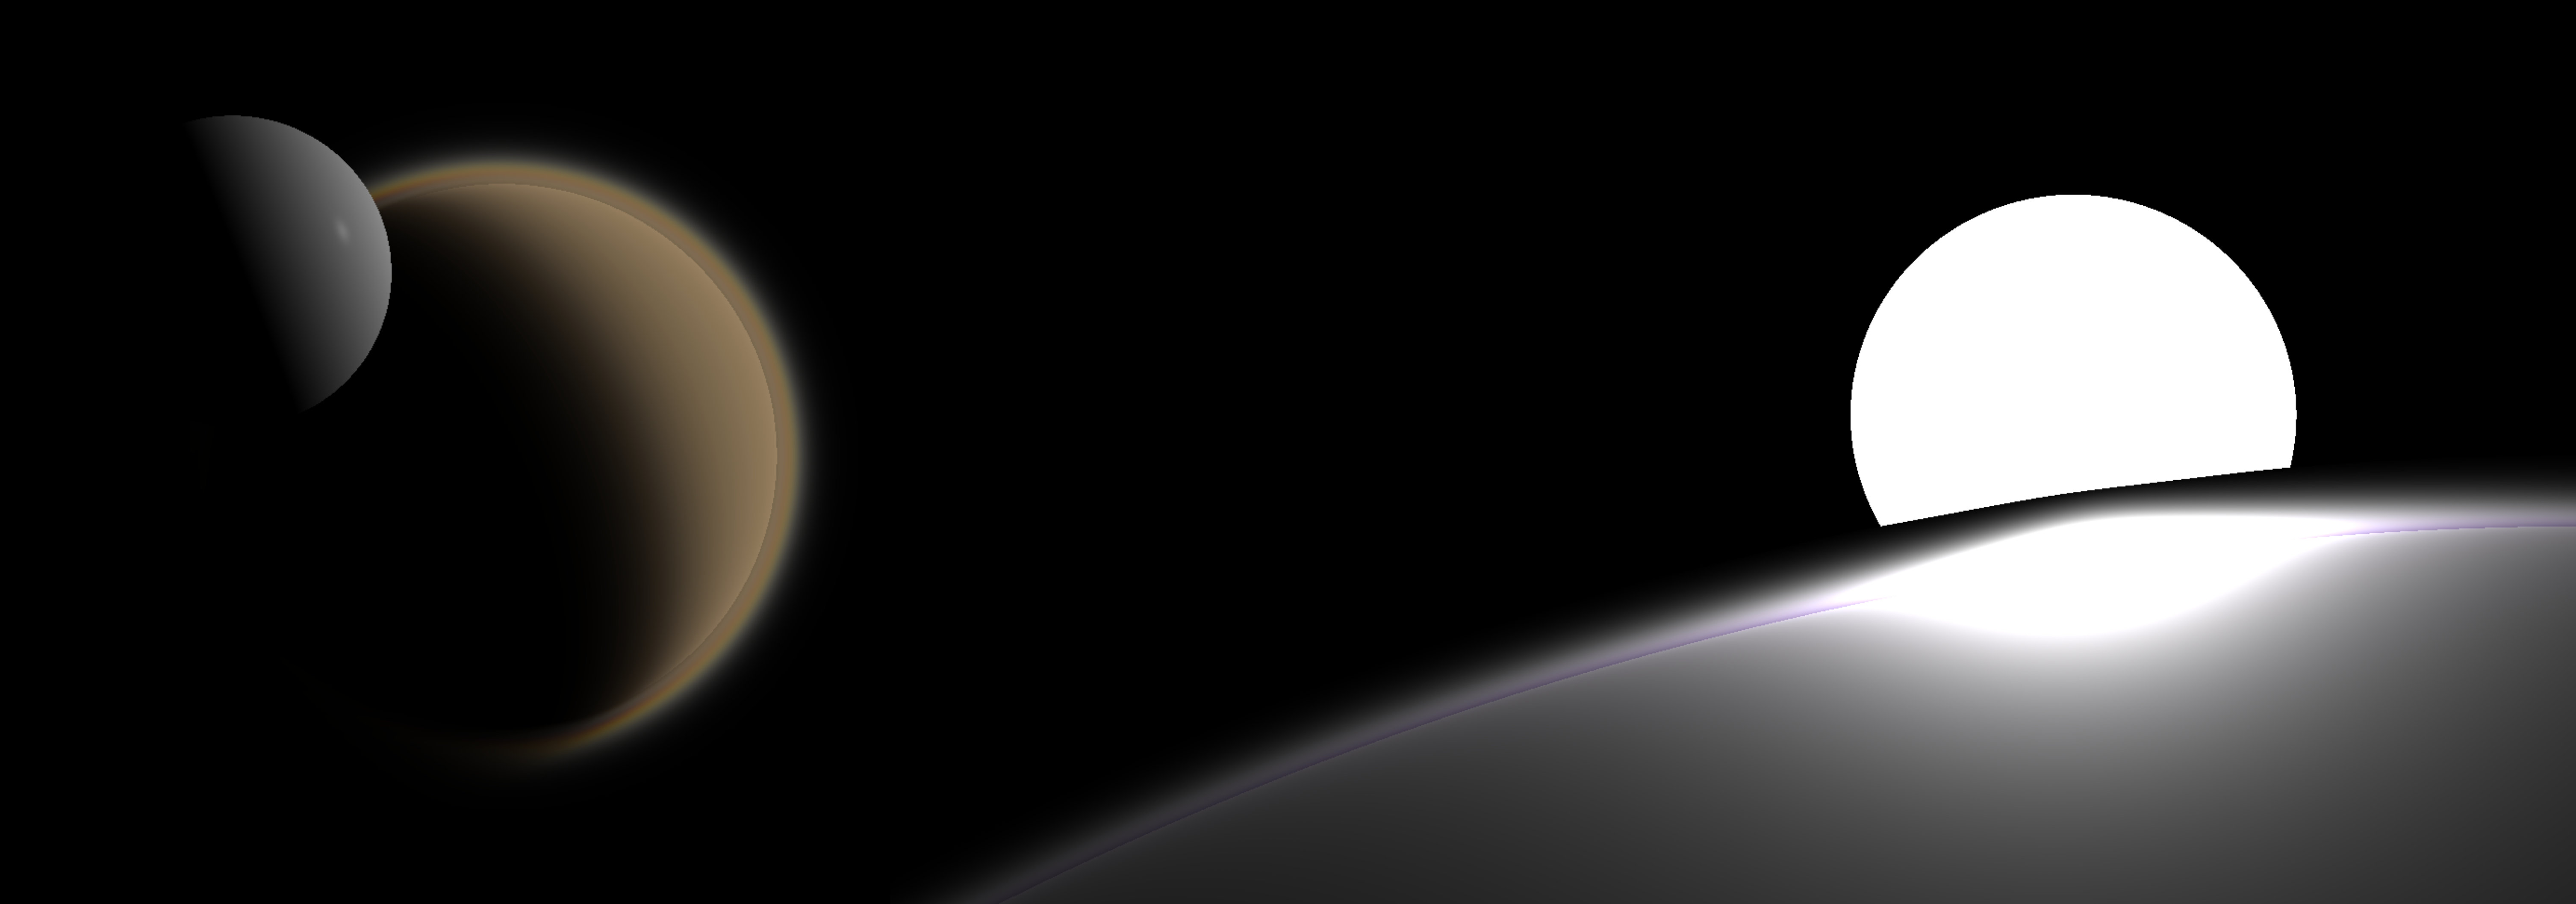
\includegraphics[width=1.0\textwidth]{./figures/occlusion.jpg}
    \caption{Stills from the shader implementation demonstrating atmospheres being partly occluded by the moon (right) and occluding the sun disk in the distance (right).}
    \label{fig:occlusion}
\end{figure}

The first step is thus to cast a ray from the camera position $P_c$ to the world position of the current fragment, where the latter is calculated in the vertex shader by ignoring the view and projection matrices.
Using an implicitly defined sphere that matches the size of the sphere mesh in the scene, we then determine the distance $P_b$ at which the ray intersects with this sphere, while no intersection results in the current fragment being discarded.
After repeating this intersection test for the surface sphere yielding $P_b$, the shader then proceeds with evaluating the in-scattering equation \eqref{eq:in} using the Riemann sum method for approximating the outer integral.
For each sampling step $P_x$ and both components (Rayleigh and Mie) separately, we determine the optical depth at the current altitude first, since it is used in both the out- and in-scattering terms.
In accordance with equation \eqref{eq:in}, the out-scattering is calculated using the Riemann approximation of the integral in equation \eqref{eq:out} for the rays $P_xP_c$ and $P_xP_a$.
This determines the amount of light that is scattered out of the ray towards the camera, which is then multiplied by the phase function $F$ and the scattering coefficient $K$ to yield the in-scattering influence on the light intensity $I_s$ emitted by sun, the only light source in the scene.
It is important to note that (especially Rayleigh) scattering affects different wavelengths of light with varying intensity, which is why all scattering terms are calculated using vectors of three components corresponding to the RGB channels.
Simultaneously, the coefficients $K$ are also expressed in this vector format, where the values are determined based on the wavelength peaks of the RGB channels as specified in the manuscript and source code of \cite{oneil_chapter_nodate}.

Concluding the approach in \cite{oneil_chapter_nodate}, the final fragment colour is then given as a combination of the in-scattering result $I_v$ and the scattered surface colour $I_e$:
\begin{equation}
    I_f(\lambda) = I_v(\lambda) + I_e(\lambda) \cdot \exp\left(-t(P_aP_b, \lambda)\right).
\end{equation}
For this project, $I_e$ is assigned a constant colour value that can be adjusted in the demo application, yet this can easily be replaced by common reflectance models such as Blinn-Phong combined with texture sampling to create a more realistic surface appearance.
\section{Results}
To visualise the output of the implemented vertex and fragment scattering shaders, a demo application for macOS was created using C++ that allows various scattering, camera, and light source parameters to be adjusted in real-time.
\begin{figure}[h!]
    \centering
    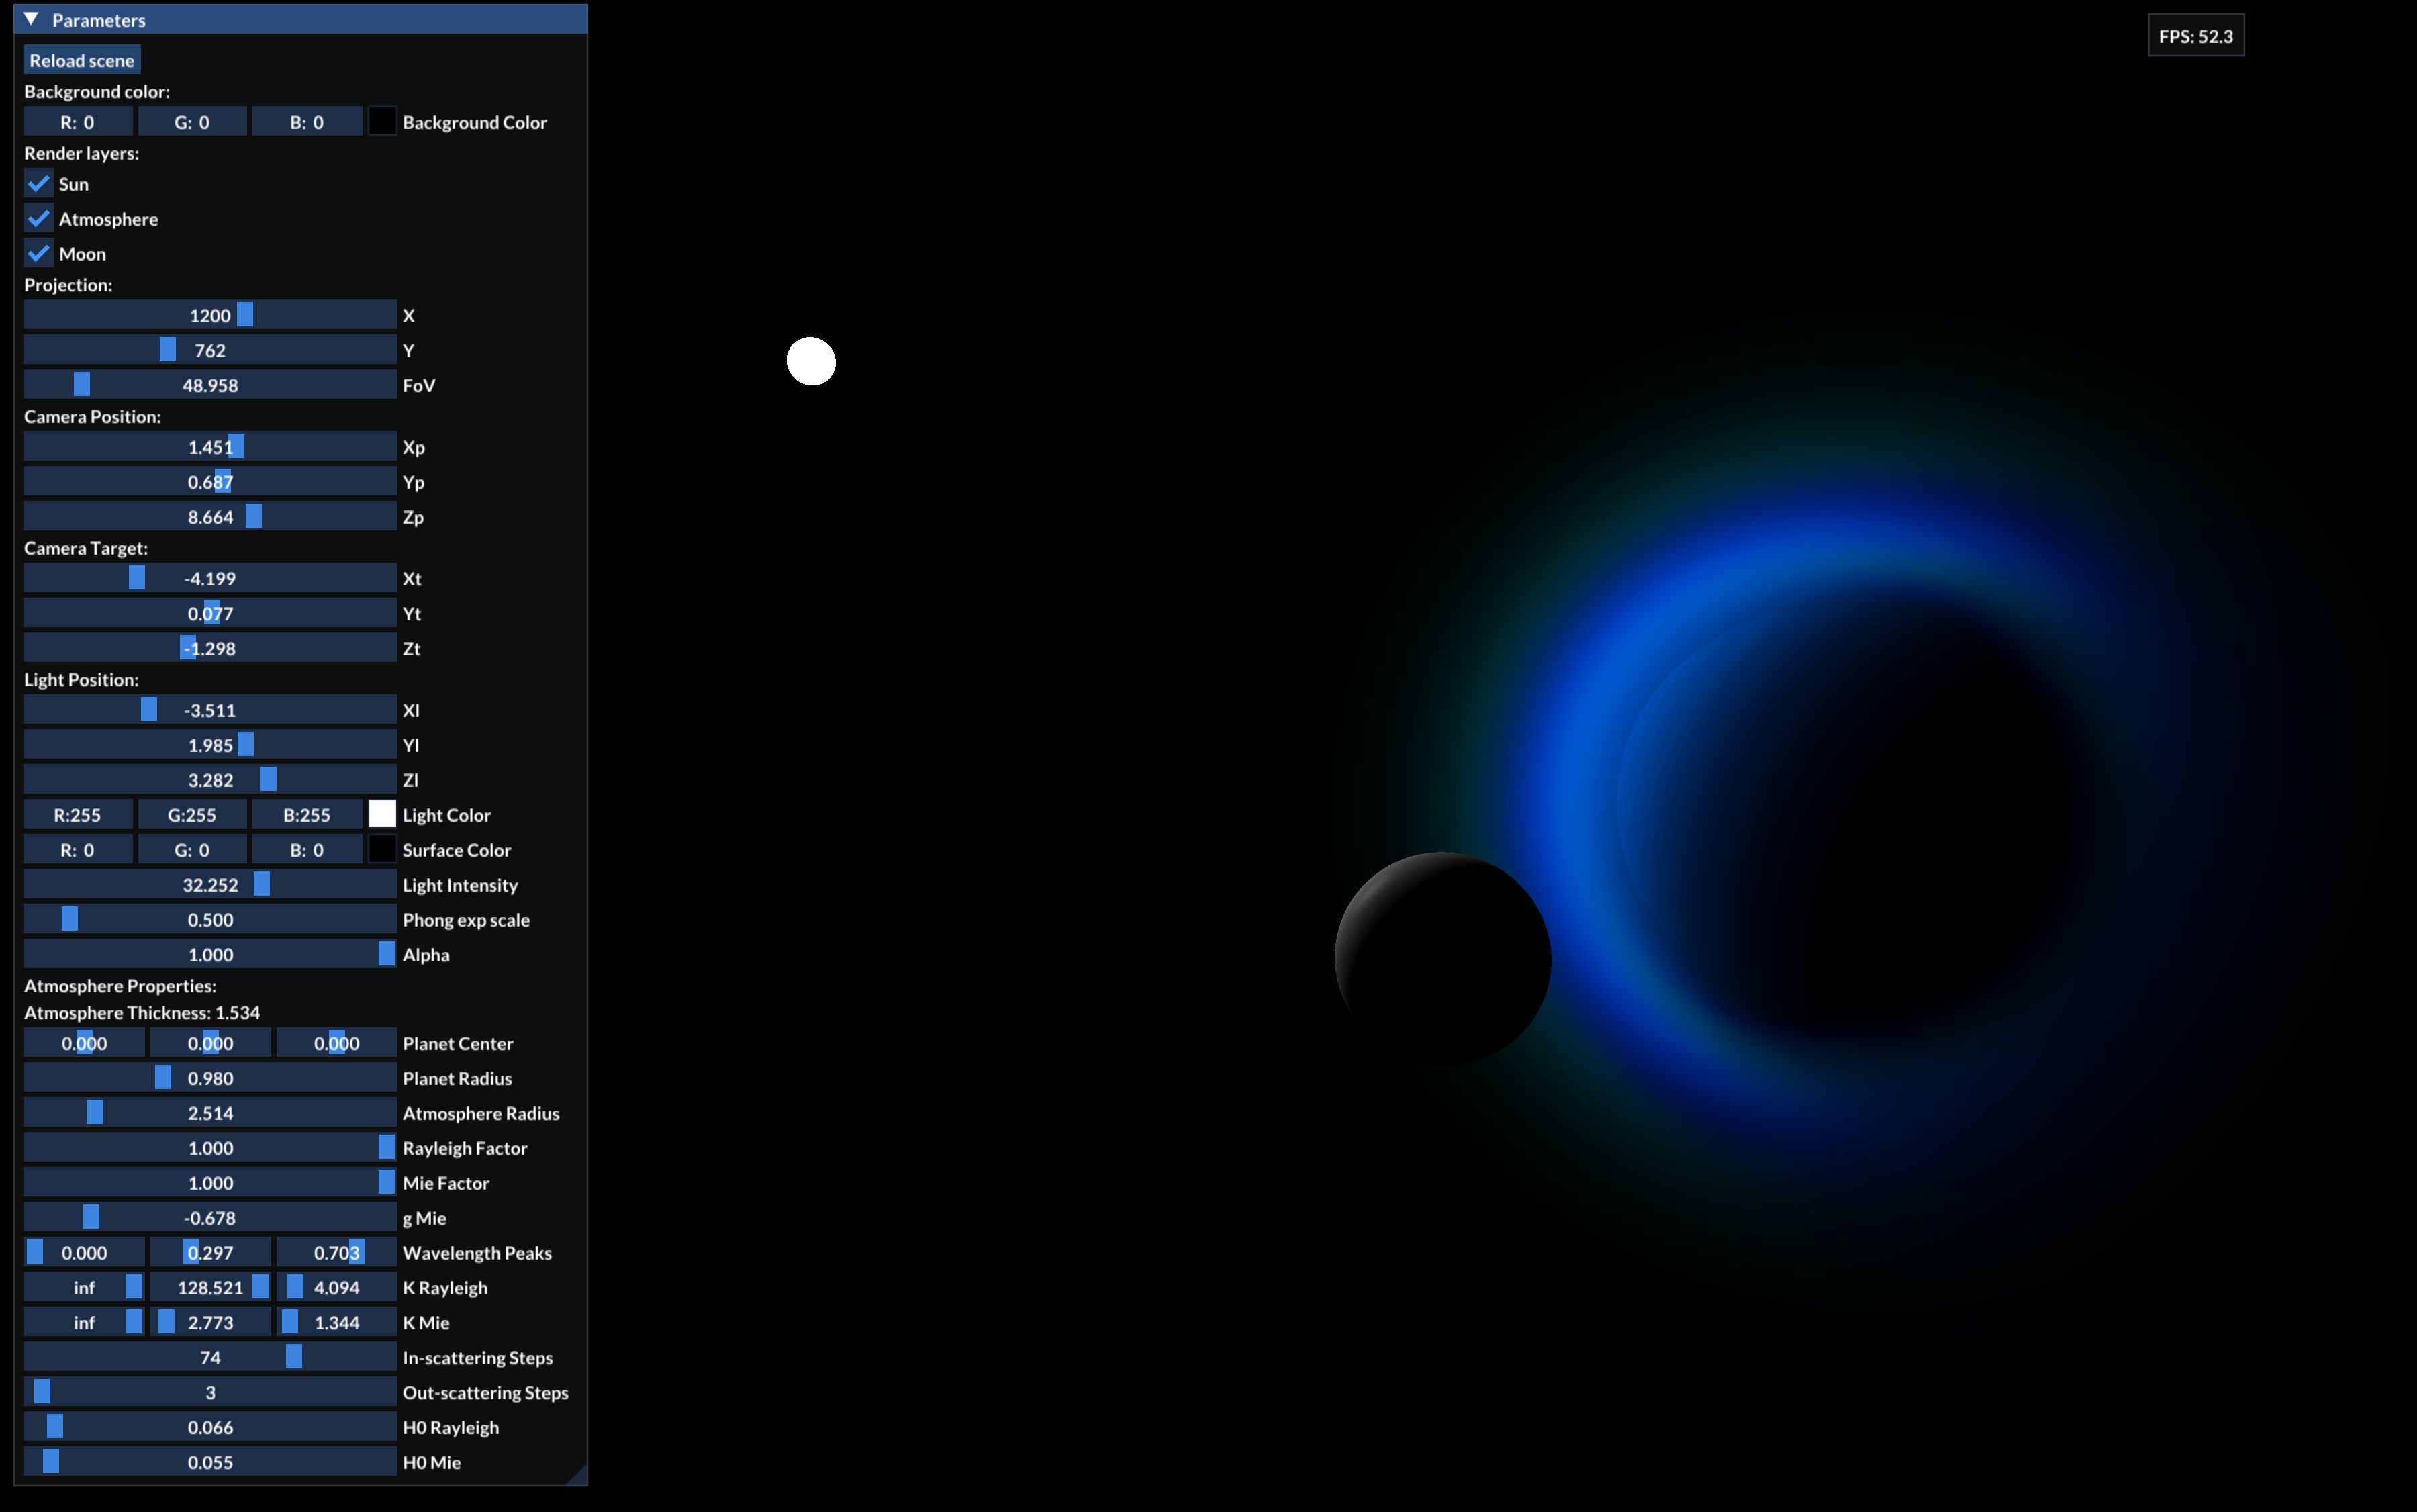
\includegraphics[width=1.0\textwidth]{./figures/demo.jpg}
    \caption{Screenshot of the demo application}
    \label{fig:occlusion}
\end{figure}
We also observe that with decreasing distance between the camera and the atmosphere, the framerate drops significantly due to the higher number of fragments that now need to  be rendered. Since the implementation discards any fragments that are not inside the atmosphere, we can avoid further unnecessary calculations.
\section{Discussion}
\newpage
\printbibliography
\newpage
\appendix
\begin{appendices}

\end{appendices}

\end{document}
